\section{Question 3}



\subsection{Testing the hypothesis}

The following hypothesis has been established based on the findings in Questions~1 and 2:
It is theoretically possible for the Scottish electricity grid to be independent and meet its electricity demand of 35,810~GWh with 100\% RE generation if:
\begin{itemize}
	\item The current RE generation mix is scaled up by 36.4\%, as shown in Table~\ref{tbl:upscale}
	\item There is PHS of 75\% efficiency with a power rating of 3.43~GW and a storage period of at least three days
\end{itemize}

EnergyPLAN was used to test this hypothesis.
To get a storage period of at least three days, 240~GWh was selected as the PHS storage capacity for a couple reasons.
Firstly, at a power rating of 3.43~GWh (to meet the peak power demand), a PHS scheme of 240~GWh storage capacity can operate continuously for about three days before the reservoirs are depleted.
Secondly, it is assumed the grid would not need to meet Scotland's peak power demand continuously for three days.
Therefore, if it is possible to limit the PHS power rating to 1.43~GW (to meet the mean winter demand), 240~GWh would yield a storage period of one week.



\subsubsection{EnergyPLAN inputs}

EnergyPLAN's UK 2020 model \citep{EnergyPLAN_UK2020} was used as the baseline model for the hypothesis.
The baseline data was amended so that there was only an electricity demand of 35.81~TWh/ year (and no heating, cooling or transport demand etc.), so that there was only RE generation (so no heat supply from district heating, combined heat and power (CHP) or heat pumps etc.) and so that there was no transmission line capacity (see Figure~\ref{fig:B02-base_load}).

\textbf{Figure~\ref{fig:B02-base_load} shows the base load inputs.}
The upscaled large scale hydro capacity of 1,829~MW was entered for Dammed Hydro Power.
The default Dammed Hydro Power efficiency was left untouched and, instead, the water supply to the Dammed Hydro was amended until the estimated annual production equalled the upscaled large scale hydro generation calculated in Question~1, i.e. 6.12~TWh/ year (see Table~\ref{tbl:upscale}).

``Condensing PP2" consists of the central power plants that generate electricity only.
PP2 was allocated 570~MW, i.e. the upscaled capacity of landfill gas, sewage sludge digestion and other biomass (see Section~\ref{sec:base_load}).
The electrical efficiency of landfill gas, sewage sludge digestion and other biomass were respectively found as ...

\begin{figure}[htbp]
	\centering
	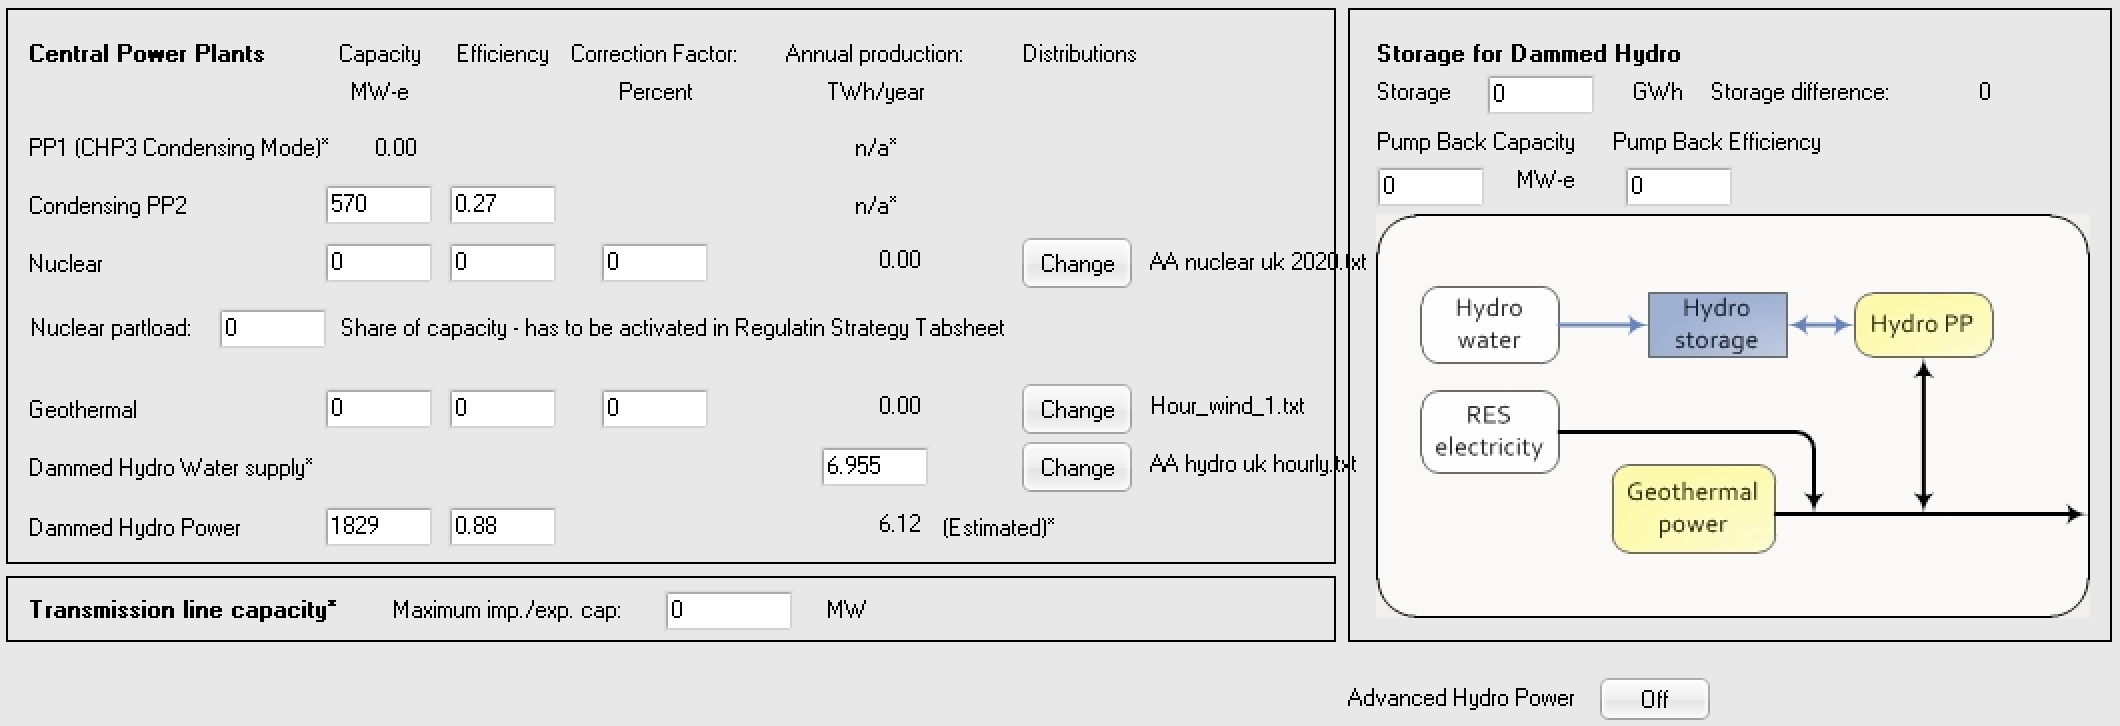
\includegraphics[width=\textwidth]{figures/B02_base_load.png}
	\rule{\textwidth}{0.5pt} % use line???
	\caption{Base load parameters and nullified transmission line capacity (screenshot of EnergyPLAN).}
	\label{fig:B02-base_load}
\end{figure}

\begin{figure}[htbp]
	\centering
	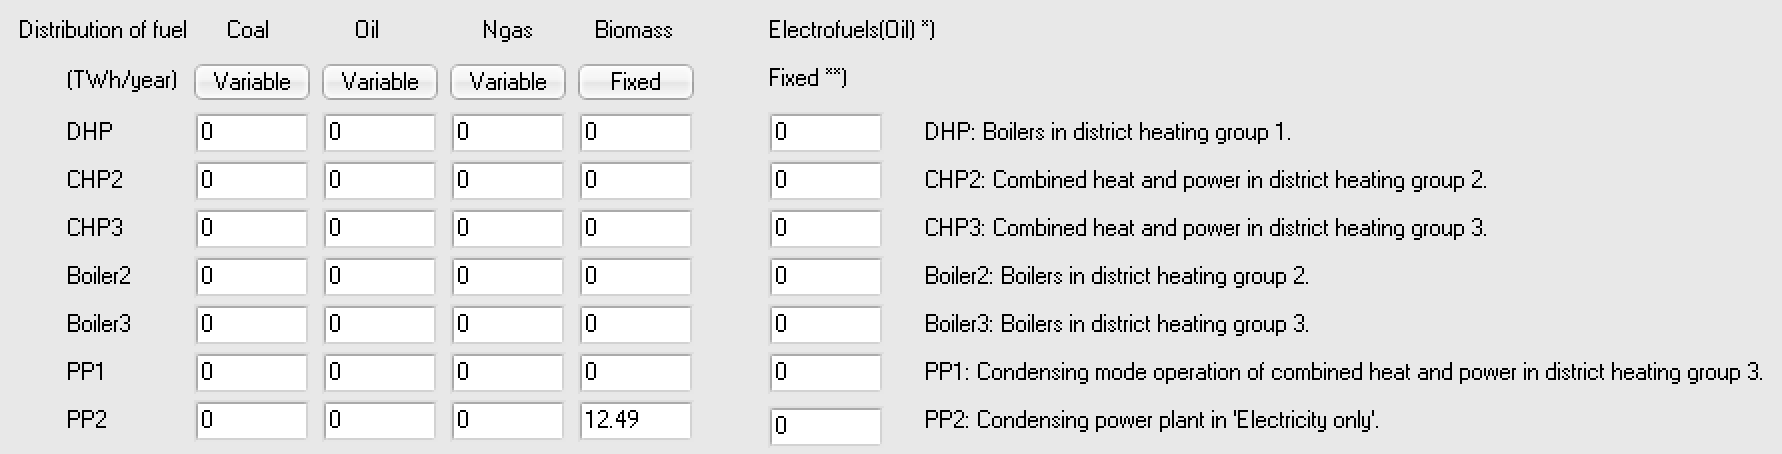
\includegraphics[width=\textwidth]{figures/B02_BM.png}
	\rule{\textwidth}{0.5pt} % use line???
	\caption{Supply of biomass to PP2.}
	\label{fig:B02-BM}
\end{figure}

\begin{figure}[htbp]
	\centering
	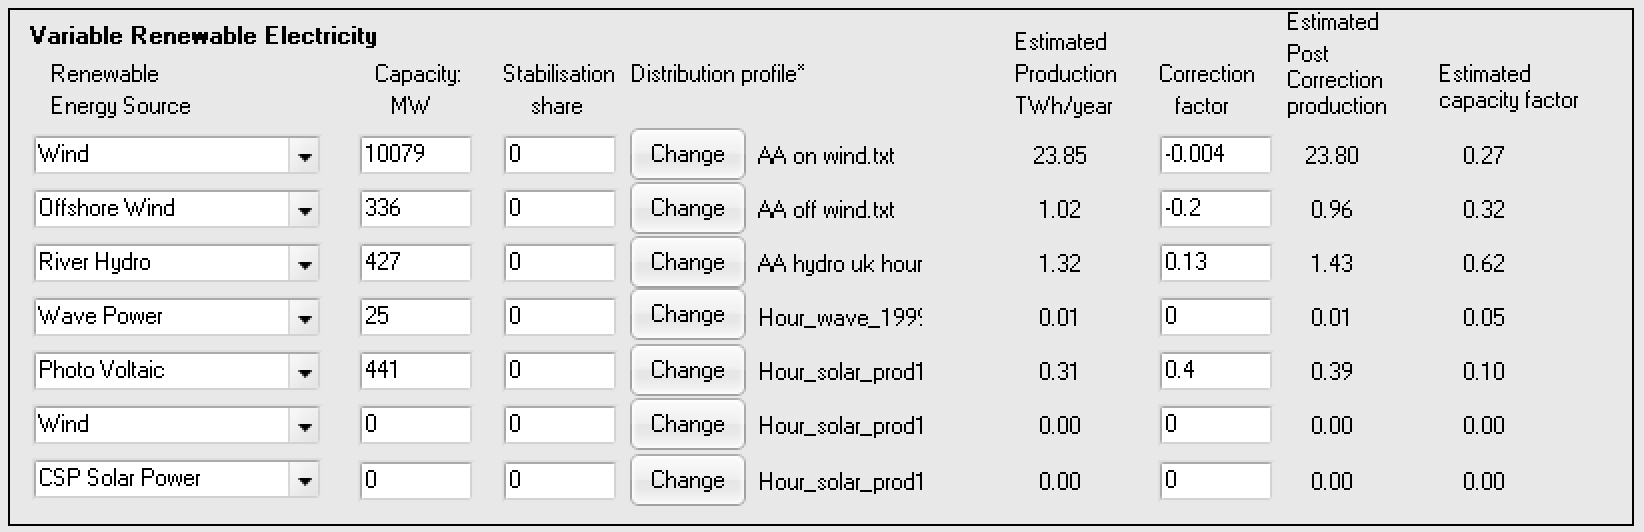
\includegraphics[width=\textwidth]{figures/B02_VRE.png}
	\rule{\textwidth}{0.5pt} % use line???
	\caption{VRE generation mix (screenshot of EnergyPLAN).}
	\label{fig:B02-VRE}
\end{figure}

\begin{figure}[htbp]
	\centering
	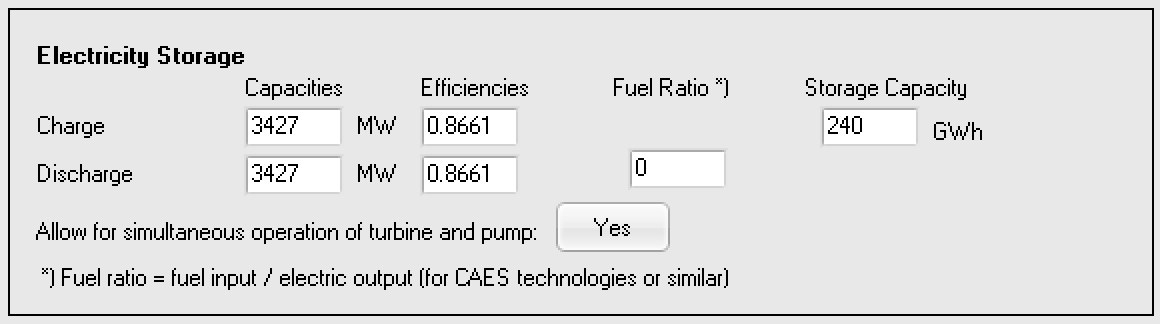
\includegraphics[width=\textwidth]{figures/B02_PHS.png}
	\rule{\textwidth}{0.5pt} % use line???
	\caption{PHS parameters.}
	\label{fig:B02-PHS}
\end{figure}










\subsection{Scenario optimisation}


\newpage
\textbf{FIDE, p. 39}

"However, if energy storage devices are
designed especially to integrate fluctuating renewable energy, there may be additional benefits when using
PHES that can charge and discharge at the same time. This can be achieved in a single PHES facility by installing
two penstocks, as displayed in Figure 21, or also by installing multiple single penstock system PHES facilities on
the same energy system i.e. one can charge while the other is discharging at the same time. By using a double
penstock system, the PHES introduces more flexibility onto the energy system and hence it can aid the
integration of more renewable energy. As a result, this operating strategy is also possible in EnergyPLAN by
selecting YES when asked “Allow for simultaneous operation of turbine and pump”"

\begin{figure}[htbp]
	\centering
	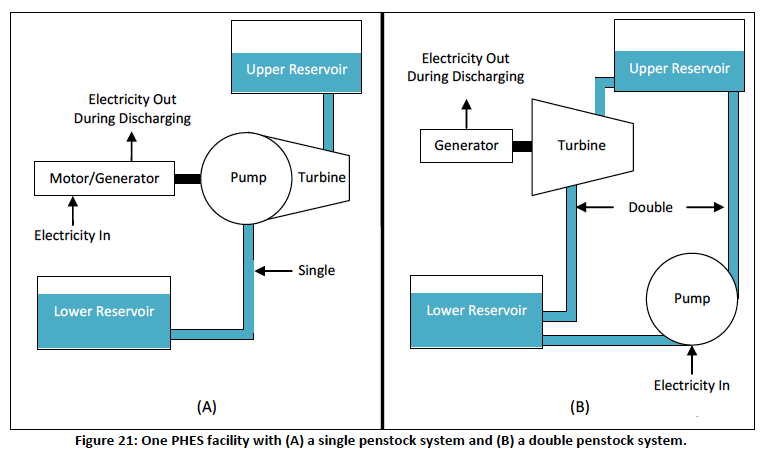
\includegraphics[width=\textwidth]{figures/Simultaneous_charge_discharge.png}
\end{figure}

"Therefore, double penstock system can achieve higher fluctuating renewable energy
penetrations at lower storage capacities than a single penstock system."